\documentclass[a4paper,12pt]{article}
%\usepackage[latin1]{inputenc}
\usepackage[spanish]{babel}
\usepackage[utf8]{inputenc}
\usepackage[usenames]{color}
%\usepackage[spanish]{babel}
\usepackage{graphicx}
\usepackage{amsmath}
\usepackage{wrapfig}
\setlength{\textheight}{250mm}
\setlength{\textwidth}{165mm}
\setlength{\topmargin}{-15mm}
\setlength{\oddsidemargin}{0pt}
\pagestyle{empty}

\begin{document}

\def\bm#1{{\mbox{\boldmath $#1$}}}
\def\eqdef{\buildrel \rm def \over =}
\def\signo{\mathop{\rm signo}\nolimits}

\mbox{}\vspace*{-20mm}

{\centering
{\small\sc Escuela Técnica Superior de Ingenieros de Caminos, Canales y Puertos (Madrid)}\\*[4mm]
{\Large\bf Método de los Elementos Finitos (Curso 21-22)}\\*[4mm]
Ejercicio 3. 
{Elementos isoparamétricos} \\*[4mm]
}

% \vspace{4mm}

% ENUNCIADO

Un panel de canto variable, con las medidas que se indican en la figura (en mm),
está empotrado en un extremo y sometido a esfuerzo cortante en el otro
extremo. El esfuerzo total aplicado es $\bm{F}=1.8$ kN, repartido a lo largo del contorno $\overline{\text{AB}}$. Las propiedades elásticas del material del panel son $E=70$ GPa y $\nu=0.33$, y su espesor es $1$ mm.
Se considerará la hipótesis de tensión plana.

La malla será de tipo estructurada, subdividiendo en 16 elementos cada lado del contorno. Se pide hacer un modelo de elementos finitos con elementos cuadriláteros de $4$ y $8$ nodos (CPS4 y CPS8 respectivamente) y contestar el cuestionario disponible en el sitio Moodle de la asignatura.


%\vspace{4cm}

\begin{figure}[h]
  \centering
  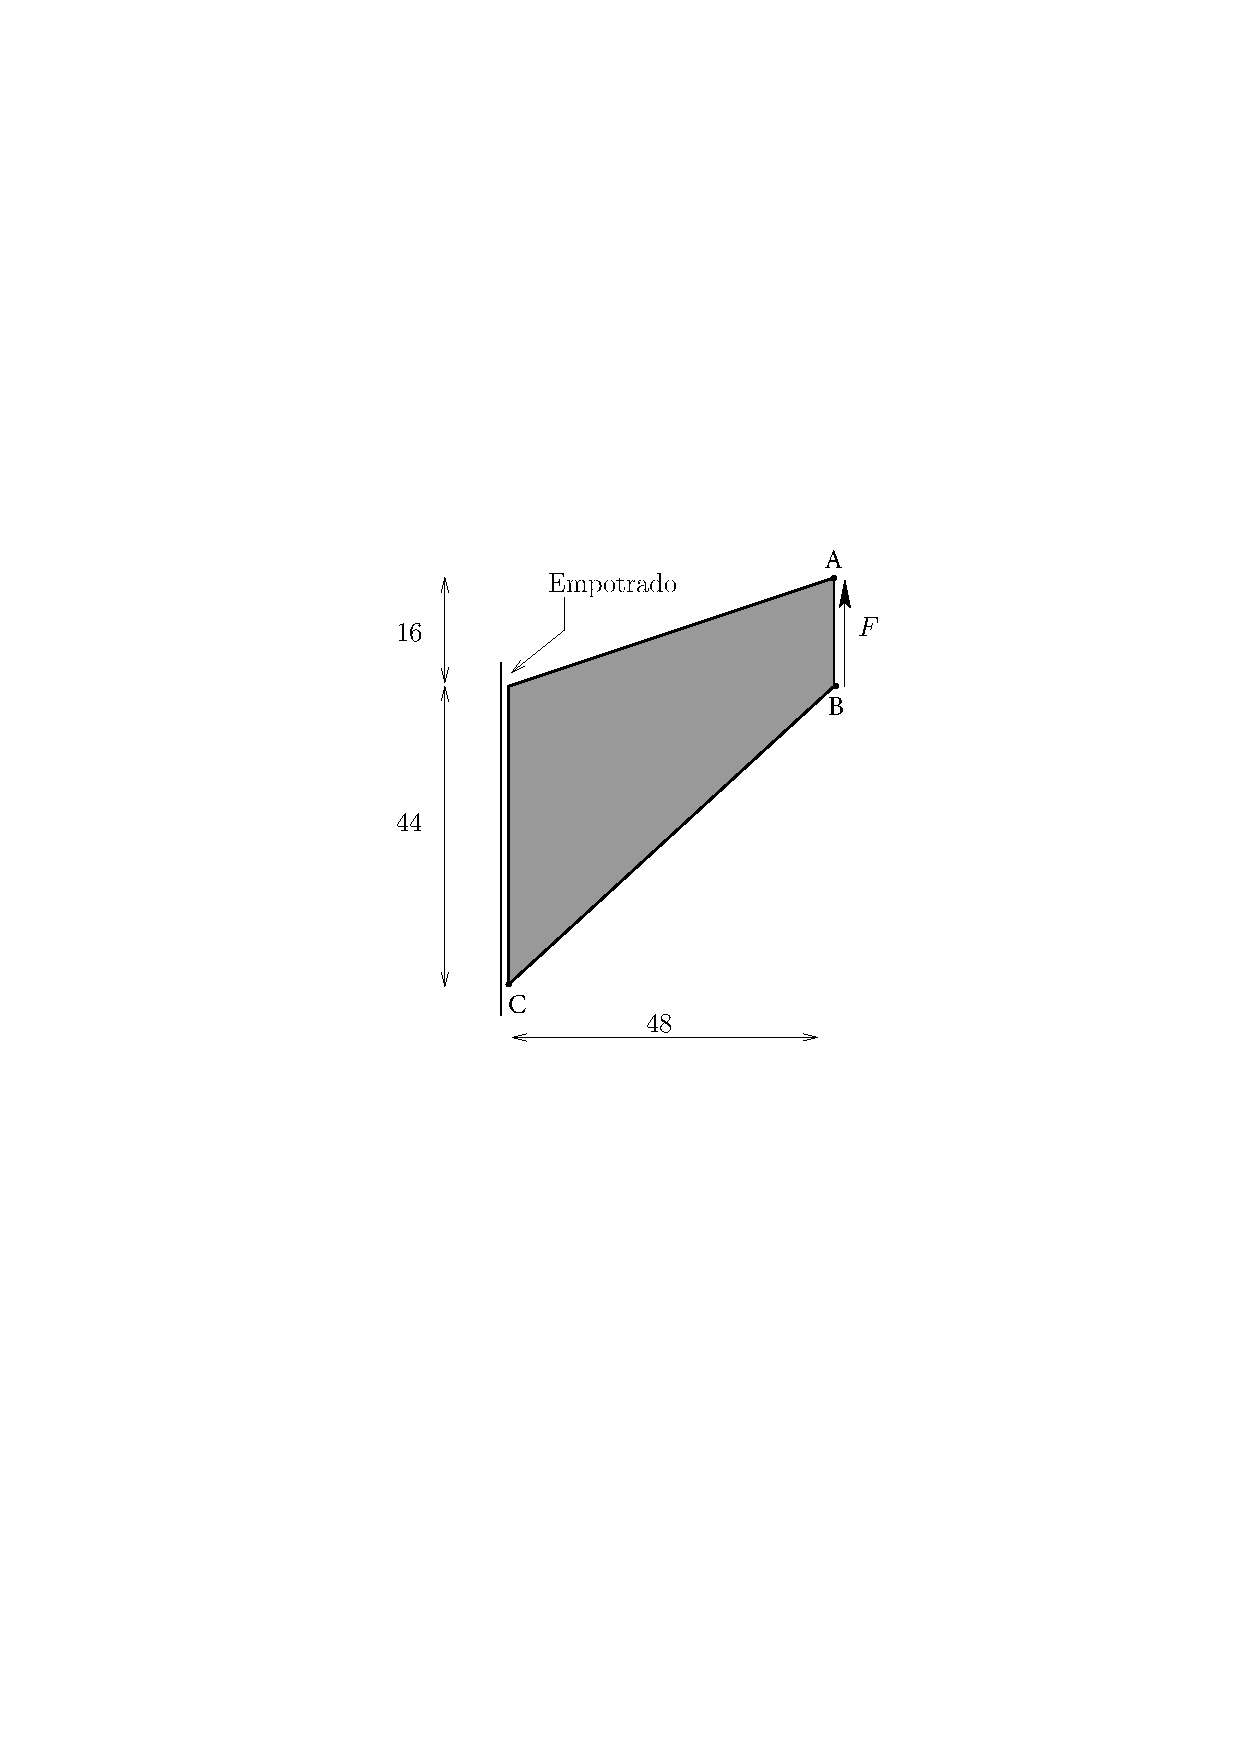
\includegraphics[width=0.5\textwidth]{CookABC.pdf}
\end{figure}

%\begin{wrapfigure}{h}
%\centering
%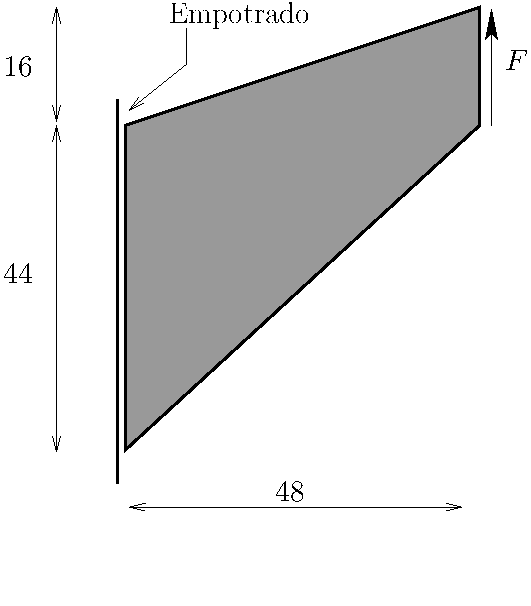
\includegraphics[width=0.5\textwidth]{cook}
%\end{wrapfigure}
\vfill
{\em \underline {Nota}: para la aplicación de la carga se utilzará el comando de Abaqus "Surface traction", seleccionando $"edit"$ para establecer la dirección en la que se aplicará.

\begin{figure}[h]
  \centering
  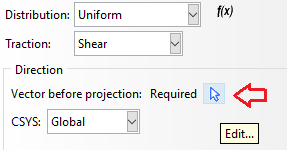
\includegraphics[width=0.3\textwidth]{surface.png}
\end{figure}

\end{document}
